\documentclass[11pt,a4paper]{article}

% ── Geometry & Layout ─────────────────────────────────────────────
\usepackage[margin=1in, headheight=14pt]{geometry}

% ── Encoding & Fonts ─────────────────────────────────────────────
\usepackage[T1]{fontenc}
\usepackage[utf8]{inputenc}
\usepackage{mathpazo}          % Palatino for body text
\usepackage{inconsolata}       % mono font for code/tables
\usepackage{microtype}         % microtypographic refinements

% ── Colour & Graphics ────────────────────────────────────────────
\usepackage[dvipsnames,svgnames,x11names]{xcolor}
\usepackage{graphicx}
\usepackage{tikz}
\usetikzlibrary{calc}

% ── Tables ────────────────────────────────────────────────────────
\usepackage{booktabs}
\usepackage{array}
\usepackage{colortbl}
\usepackage{multirow}
\usepackage{makecell}

% ── Math, Captions, Floats ────────────────────────────────────────
\usepackage{amsmath,amssymb}
\usepackage{float}
\usepackage[font=small,labelfont=bf,labelsep=period]{caption}
\usepackage{subcaption}

% ── Headers & Footers ────────────────────────────────────────────
\usepackage{fancyhdr}
\usepackage{lastpage}

% ── Boxes & Highlights ───────────────────────────────────────────
\usepackage[most]{tcolorbox}

% ── Section Styling ──────────────────────────────────────────────
\usepackage{titlesec}

% ── Hyperlinks ───────────────────────────────────────────────────
\usepackage[colorlinks=true,linkcolor=NavyBlue,citecolor=NavyBlue,urlcolor=RoyalBlue]{hyperref}

% ── Enumeration ──────────────────────────────────────────────────
\usepackage{enumitem}

% ═══════════════════════════════════════════════════════════════════
%                       COLOUR PALETTE
% ═══════════════════════════════════════════════════════════════════
\definecolor{BilkentBlue}{HTML}{004B87}
\definecolor{AccentOrange}{HTML}{E8702A}
\definecolor{LightBG}{HTML}{F5F7FA}
\definecolor{TableHead}{HTML}{DBEAFE}
\definecolor{TableAlt}{HTML}{F0F5FF}
\definecolor{FindingGreen}{HTML}{E8F5E9}
\definecolor{FindingBorder}{HTML}{43A047}
\definecolor{WarningYellow}{HTML}{FFF8E1}
\definecolor{WarningBorder}{HTML}{F9A825}

% ═══════════════════════════════════════════════════════════════════
%                       PARAGRAPH SETTINGS
% ═══════════════════════════════════════════════════════════════════
\setlength{\parindent}{0pt}
\setlength{\parskip}{0.5em}

% ═══════════════════════════════════════════════════════════════════
%                       SECTION FORMATTING
% ═══════════════════════════════════════════════════════════════════
\titleformat{\section}
  {\Large\bfseries\color{BilkentBlue}}
  {\thesection}{0.7em}{}
  [\vspace{-0.3em}{\color{AccentOrange}\titlerule[1.8pt]}]

\titleformat{\subsection}
  {\large\bfseries\color{BilkentBlue!80!black}}
  {\thesubsection}{0.6em}{}

% ═══════════════════════════════════════════════════════════════════
%                    HEADER / FOOTER STYLE
% ═══════════════════════════════════════════════════════════════════
\pagestyle{fancy}
\fancyhf{}
\renewcommand{\headrulewidth}{0.4pt}
\fancyhead[L]{\small\color{BilkentBlue}\textsc{IE\,306 -- Assignment 2}}
\fancyhead[R]{\small\color{BilkentBlue}\textsc{Group Mehmet}}
\fancyfoot[C]{\small\color{gray}\thepage\ / \pageref{LastPage}}

% ═══════════════════════════════════════════════════════════════════
%                    CALLOUT BOX STYLES
% ═══════════════════════════════════════════════════════════════════
\newtcolorbox{findingbox}[1][]{%
  enhanced,
  colback=FindingGreen,
  colframe=FindingBorder,
  boxrule=0.8pt,
  left=8pt, right=8pt, top=6pt, bottom=6pt,
  arc=3pt,
  fonttitle=\bfseries\color{FindingBorder},
  title={#1},
  before upper={\setlength{\parskip}{0.4em}}
}

\newtcolorbox{cautionbox}[1][]{%
  enhanced,
  colback=WarningYellow,
  colframe=WarningBorder,
  boxrule=0.8pt,
  left=8pt, right=8pt, top=6pt, bottom=6pt,
  arc=3pt,
  fonttitle=\bfseries\color{WarningBorder},
  title={#1},
  before upper={\setlength{\parskip}{0.4em}}
}

\newtcolorbox{infobox}[1][]{%
  enhanced,
  colback=LightBG,
  colframe=BilkentBlue,
  boxrule=0.8pt,
  left=8pt, right=8pt, top=6pt, bottom=6pt,
  arc=3pt,
  fonttitle=\bfseries\color{BilkentBlue},
  title={#1},
  before upper={\setlength{\parskip}{0.4em}}
}

% ═══════════════════════════════════════════════════════════════════
%                         DOCUMENT
% ═══════════════════════════════════════════════════════════════════
\begin{document}

% ──────────────────────── TITLE PAGE ──────────────────────────────
\thispagestyle{empty}
\begin{tikzpicture}[remember picture, overlay]
  % Top accent band
  \fill[BilkentBlue] (current page.north west) rectangle
    ([yshift=-4.5cm]current page.north east);
  % Accent stripe
  \fill[AccentOrange] ([yshift=-4.5cm]current page.north west) rectangle
    ([yshift=-4.8cm]current page.north east);
\end{tikzpicture}

\vspace*{-1.2cm}

\begin{center}
  {\color{white}\LARGE\textsc{IE\,306 -- Systems Simulation}}\\[6pt]
  {\color{white}\Large Spring 2026}
\end{center}

\vspace{3.5cm}

\begin{center}
  {\Huge\bfseries\color{BilkentBlue} Coordinated Traffic\\[4pt]
   Corridor Simulation}\\[1.2cm]
  {\Large\color{BilkentBlue!70!black} Assignment~2}\\[2cm]
  {\large
    \begin{tabular}{c}
      \textbf{Group Mehmet}\\[8pt]
      Mehmet Kaan \"Unsel\\[3pt]
      Ali Ayhan G\"under\\[3pt]
      Mustafa \"Ozt\"urkmen
    \end{tabular}}
\end{center}

\vfill

\begin{center}
  \textcolor{gray}{\small Submitted: Spring 2026}
\end{center}

\newpage

% ──────────────────── TABLE OF CONTENTS ───────────────────────────
\tableofcontents
\newpage

% ══════════════════════════════════════════════════════════════════
%  1. MODEL LOGIC AND ASSUMPTIONS
% ══════════════════════════════════════════════════════════════════
\section{Model Logic and Assumptions}
\label{sec:model}

\subsection{Network Topology}

We modelled the corridor as a discrete-event system in SimPy with two intersections, A~and~B, a one-directional A\,--\,B link, and four active approaches: A~N/S, A~W/E, B~N/S, and B~W/E. Southbound entries at~A follow a Poisson process with rate $\lambda = 900\;\text{veh/h}$ and are split into cars, buses, and emergency vehicles using the required proportions. Independent W/E arrivals at A and B each follow Poisson processes with rate $\lambda_{\mathrm{WE}} = 400\;\text{veh/h}$. Turning decisions are sampled independently at A and B according to the assignment probabilities.

\subsection{Signal Control}

Each intersection is controlled by a \textbf{fixed-time two-phase signal cycle}: N/S green $\rightarrow$ all-red clearance $\rightarrow$ W/E green $\rightarrow$ all-red clearance. The coordinated scenario uses the required \textbf{20\,s offset} so that B's N/S green starts one free-flow travel time after A's N/S green.

\subsection{Queue Discipline and Priority}

Queue discipline is \emph{explicit} rather than hidden inside a resource abstraction because service depends jointly on signal state, queue priority, and downstream link availability.

\begin{infobox}[Priority Scheme]
\begin{enumerate}[leftmargin=1.2em,itemsep=2pt]
  \item \textbf{Emergency vehicles} -- highest priority (preemptive trigger)
  \item \textbf{Buses} -- second priority (non-preemptive; applied when next service starts)
  \item \textbf{Regular cars} -- lowest priority
\end{enumerate}
\end{infobox}

\subsection{A\,--\,B Link Model}

The A\,--\,B link is represented as a finite-capacity point queue with $N_{\max}=40$ and travel time
\[
  t_{\text{travel}}(n) = \frac{20}{1 - n/40}\,,
\]
augmented by a small multiplicative noise term sampled from a dedicated RNG stream. Non-emergency northbound vehicles at~A can only enter the link when A~is in N/S green and the link is not full. Emergency vehicles bypass the blocking rule exactly as required and can enter even if the link is already full; they still increase the link occupancy.

\subsection{Emergency Preemption Protocol}

Emergency preemption is implemented by:
\begin{enumerate}[leftmargin=1.2em,itemsep=2pt]
  \item Interrupting the current non-N/S phase,
  \item Inserting a 4\,s all-red clearance,
  \item Forcing a 10\,s N/S green, and
  \item Resuming the interrupted phase remainder.
\end{enumerate}
We report \emph{recovery time} as the resumed interrupted-phase remainder after the emergency green ends. This matches the assignment definition more closely than timing from the original preemption trigger.

\subsection{Warm-Up Treatment}

\begin{cautionbox}[Warm-Up Protocol]
Time-persistent KPIs (queues and link occupancy) are integrated only over $t \ge 900\;\text{s}$. Through-delay observations are recorded only for southbound vehicles that entered the system after warm-up; W/E delay observations are recorded only for W/E arrivals that joined after warm-up. Throughput counts all northbound exits occurring after warm-up because it is a post-warm-up \emph{flow-rate} KPI.
\end{cautionbox}

\subsection{Random-Number Streams}

\begin{table}[H]
\centering
\caption{Random-number stream assignment. All streams are created from \texttt{numpy.random.SeedSequence([20260407,\;scenario\_id,\;replication\_id])}.}
\label{tab:rng}
\small
\rowcolors{2}{TableAlt}{white}
\begin{tabular}{c l}
\toprule
\rowcolor{TableHead}
\textbf{Stream} & \textbf{Purpose} \\
\midrule
0 & Southbound interarrival times at A \\
1 & W/E interarrival times at A \\
2 & W/E interarrival times at B \\
3 & Southbound vehicle classification \\
4 & Turning decisions at A \\
5 & Turning decisions at B \\
6 & Service times at A \\
7 & Service times at B \\
8 & Link travel-time noise \\
\bottomrule
\end{tabular}
\end{table}

\subsection{Conceptual Model}

\begin{figure}[H]
\centering
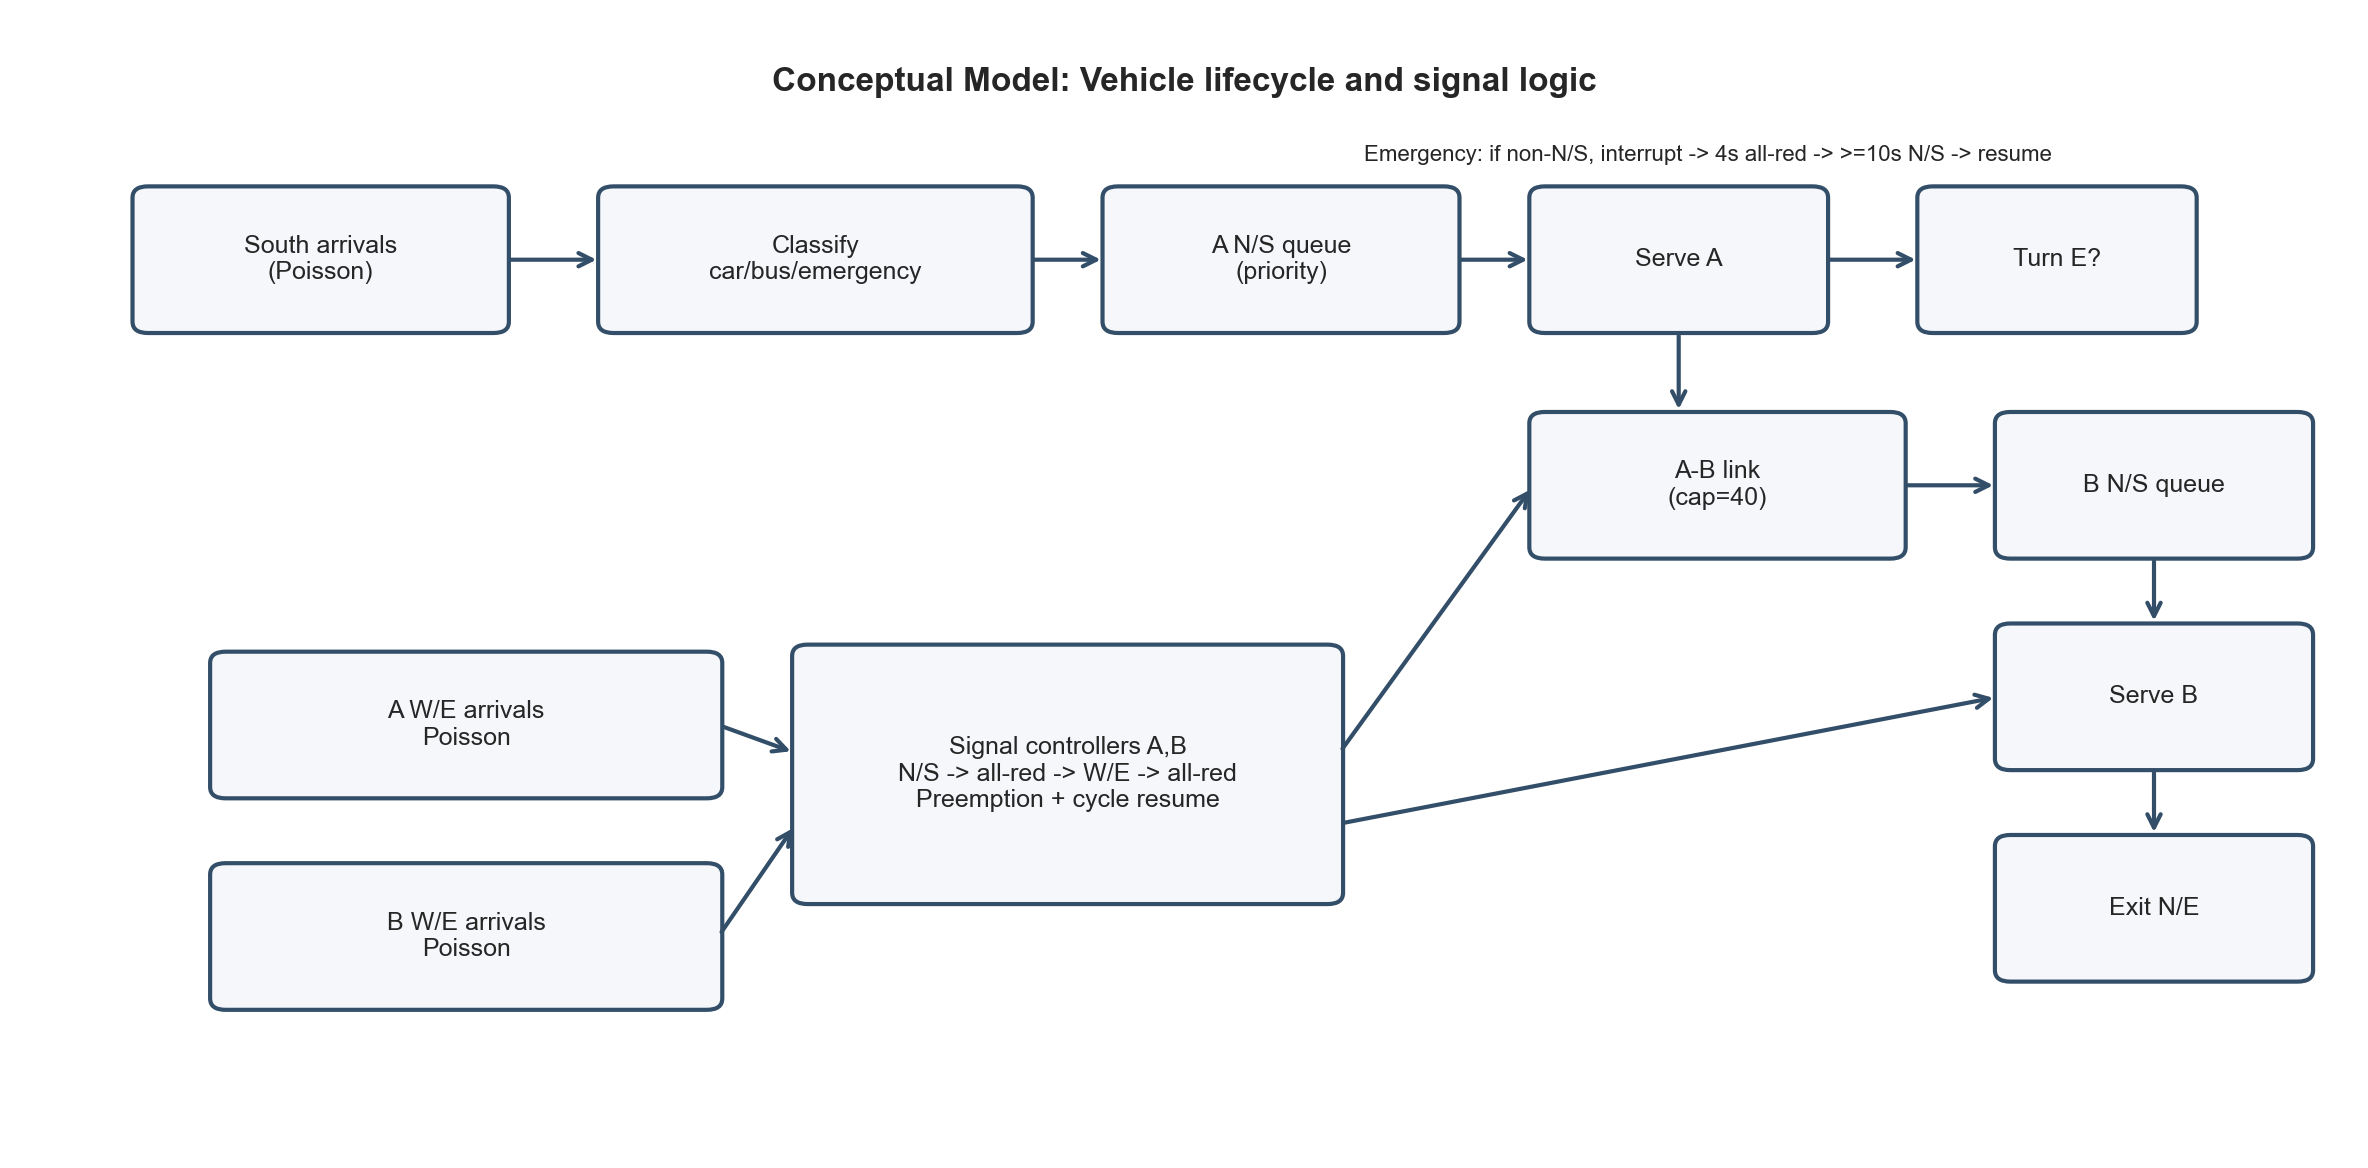
\includegraphics[width=0.92\textwidth]{outputs/conceptual_model.png}
\caption{Conceptual model diagram generated from the simulation notebook, illustrating the two-intersection corridor with the A\,--\,B link, signal phases, and vehicle routing logic.}
\label{fig:concept}
\end{figure}

% ══════════════════════════════════════════════════════════════════
%  2. EXPERIMENTAL DESIGN
% ══════════════════════════════════════════════════════════════════
\section{Experimental Design}
\label{sec:design}

We ran the three required scenarios:

\begin{table}[H]
\centering
\caption{Scenario definitions.}
\label{tab:scenarios}
\small
\rowcolors{2}{TableAlt}{white}
\begin{tabular}{c l c c}
\toprule
\rowcolor{TableHead}
\textbf{ID} & \textbf{Description} & \textbf{Coordination} & \textbf{Emergencies} \\
\midrule
S1 & Uncoordinated, no emergencies & \textsf{Off}  & \textsf{Off} \\
S2 & Coordinated, no emergencies   & \textsf{On}   & \textsf{Off} \\
S3 & Coordinated, with emergencies & \textsf{On}   & \textsf{On}  \\
\bottomrule
\end{tabular}
\end{table}

Each scenario was simulated for \textbf{7\,200\,s} (2 hours), the first \textbf{900\,s} were discarded as warm-up, and \textbf{20 independent replications} were run. Point estimates are reported as replication means and 95\,\% confidence intervals are computed as $\bar{x} \pm 1.96 \times s / \sqrt{n}$.

% ══════════════════════════════════════════════════════════════════
%  3. RESULTS
% ══════════════════════════════════════════════════════════════════
\section{Results}
\label{sec:results}

Table~\ref{tab:main-kpis} summarises the main operational KPIs. Table~\ref{tab:queue-kpis} reports average and maximum queue lengths for each approach. Figures~\ref{fig:ci} and~\ref{fig:queue} visualise the same results using compact comparative plots saved by the notebook.

% ── Main KPI Table ────────────────────────────────────────────────
\begin{table}[H]
\centering
\caption{Main KPI summary -- mean\;[95\,\% CI].}
\label{tab:main-kpis}
\small
\rowcolors{2}{TableAlt}{white}
\begin{tabular}{>{\raggedright\arraybackslash}p{4.5cm} c c c}
\toprule
\rowcolor{TableHead}
\textbf{KPI} & \textbf{S1 Uncoord.} & \textbf{S2 Coord.} & \textbf{S3 Coord.\,+\,Emerg.} \\
\midrule
Avg delay (through S$\rightarrow$N) [s]
  & 121.57 \scriptsize[102.45,\,140.69]
  & 95.58  \scriptsize[83.73,\,107.44]
  & 70.41  \scriptsize[61.95,\,78.88] \\
Avg delay (W$\rightarrow$E) [s]
  & 21.75  \scriptsize[21.38,\,22.12]
  & 21.47  \scriptsize[21.09,\,21.85]
  & 22.78  \scriptsize[22.40,\,23.15] \\
Throughput NB at B [veh/h]
  & 504.60 \scriptsize[498.23,\,510.97]
  & 503.37 \scriptsize[495.48,\,511.26]
  & 510.63 \scriptsize[501.90,\,519.35] \\
Avg link occupancy [veh]
  & 4.16   \scriptsize[4.10,\,4.22]
  & 4.11   \scriptsize[4.06,\,4.16]
  & 4.11   \scriptsize[4.06,\,4.17] \\
Blocking frequency [frac.\,cycles]
  & 0.000  \scriptsize[0.000,\,0.000]
  & 0.000  \scriptsize[0.000,\,0.000]
  & 0.000  \scriptsize[0.000,\,0.000] \\
Preemptions per replication
  & 0.00   \scriptsize[0.00,\,0.00]
  & 0.00   \scriptsize[0.00,\,0.00]
  & 54.05  \scriptsize[51.29,\,56.81] \\
Recovery time [s]
  & 0.00   \scriptsize[0.00,\,0.00]
  & 0.00   \scriptsize[0.00,\,0.00]
  & 15.95  \scriptsize[15.36,\,16.53] \\
\bottomrule
\end{tabular}
\end{table}

% ── Queue KPI Table ───────────────────────────────────────────────
\begin{table}[H]
\centering
\caption{Queue-length KPI summary -- mean\;[95\,\% CI].}
\label{tab:queue-kpis}
\small
\rowcolors{2}{TableAlt}{white}
\begin{tabular}{>{\raggedright\arraybackslash}p{4.2cm} c c c}
\toprule
\rowcolor{TableHead}
\textbf{KPI} & \textbf{S1 Uncoord.} & \textbf{S2 Coord.} & \textbf{S3 Coord.\,+\,Emerg.} \\
\midrule
Avg queue A\,N/S [veh]
  & 24.34 \scriptsize[19.48,\,29.20]
  & 21.29 \scriptsize[18.24,\,24.33]
  & 13.25 \scriptsize[11.19,\,15.31] \\
Max queue A\,N/S [veh]
  & 62.10 \scriptsize[53.22,\,70.98]
  & 56.60 \scriptsize[50.05,\,63.15]
  & 41.90 \scriptsize[36.35,\,47.45] \\
Avg queue B\,N/S [veh]
  & 4.57  \scriptsize[4.39,\,4.75]
  & 2.02  \scriptsize[1.90,\,2.14]
  & 3.22  \scriptsize[2.85,\,3.58] \\
Max queue B\,N/S [veh]
  & 18.65 \scriptsize[17.56,\,19.74]
  & 13.30 \scriptsize[11.93,\,14.67]
  & 19.25 \scriptsize[18.13,\,20.37] \\
Avg queue A\,W/E [veh]
  & 2.40  \scriptsize[2.32,\,2.49]
  & 2.40  \scriptsize[2.31,\,2.49]
  & 2.58  \scriptsize[2.49,\,2.68] \\
Max queue A\,W/E [veh]
  & 12.60 \scriptsize[11.78,\,13.42]
  & 13.30 \scriptsize[12.23,\,14.37]
  & 14.10 \scriptsize[13.28,\,14.92] \\
Avg queue B\,W/E [veh]
  & 2.45  \scriptsize[2.36,\,2.54]
  & 2.39  \scriptsize[2.33,\,2.45]
  & 2.53  \scriptsize[2.44,\,2.62] \\
Max queue B\,W/E [veh]
  & 12.80 \scriptsize[12.12,\,13.48]
  & 12.85 \scriptsize[11.79,\,13.91]
  & 12.65 \scriptsize[12.22,\,13.08] \\
\bottomrule
\end{tabular}
\end{table}

% ── Figures ───────────────────────────────────────────────────────
\begin{figure}[H]
\centering
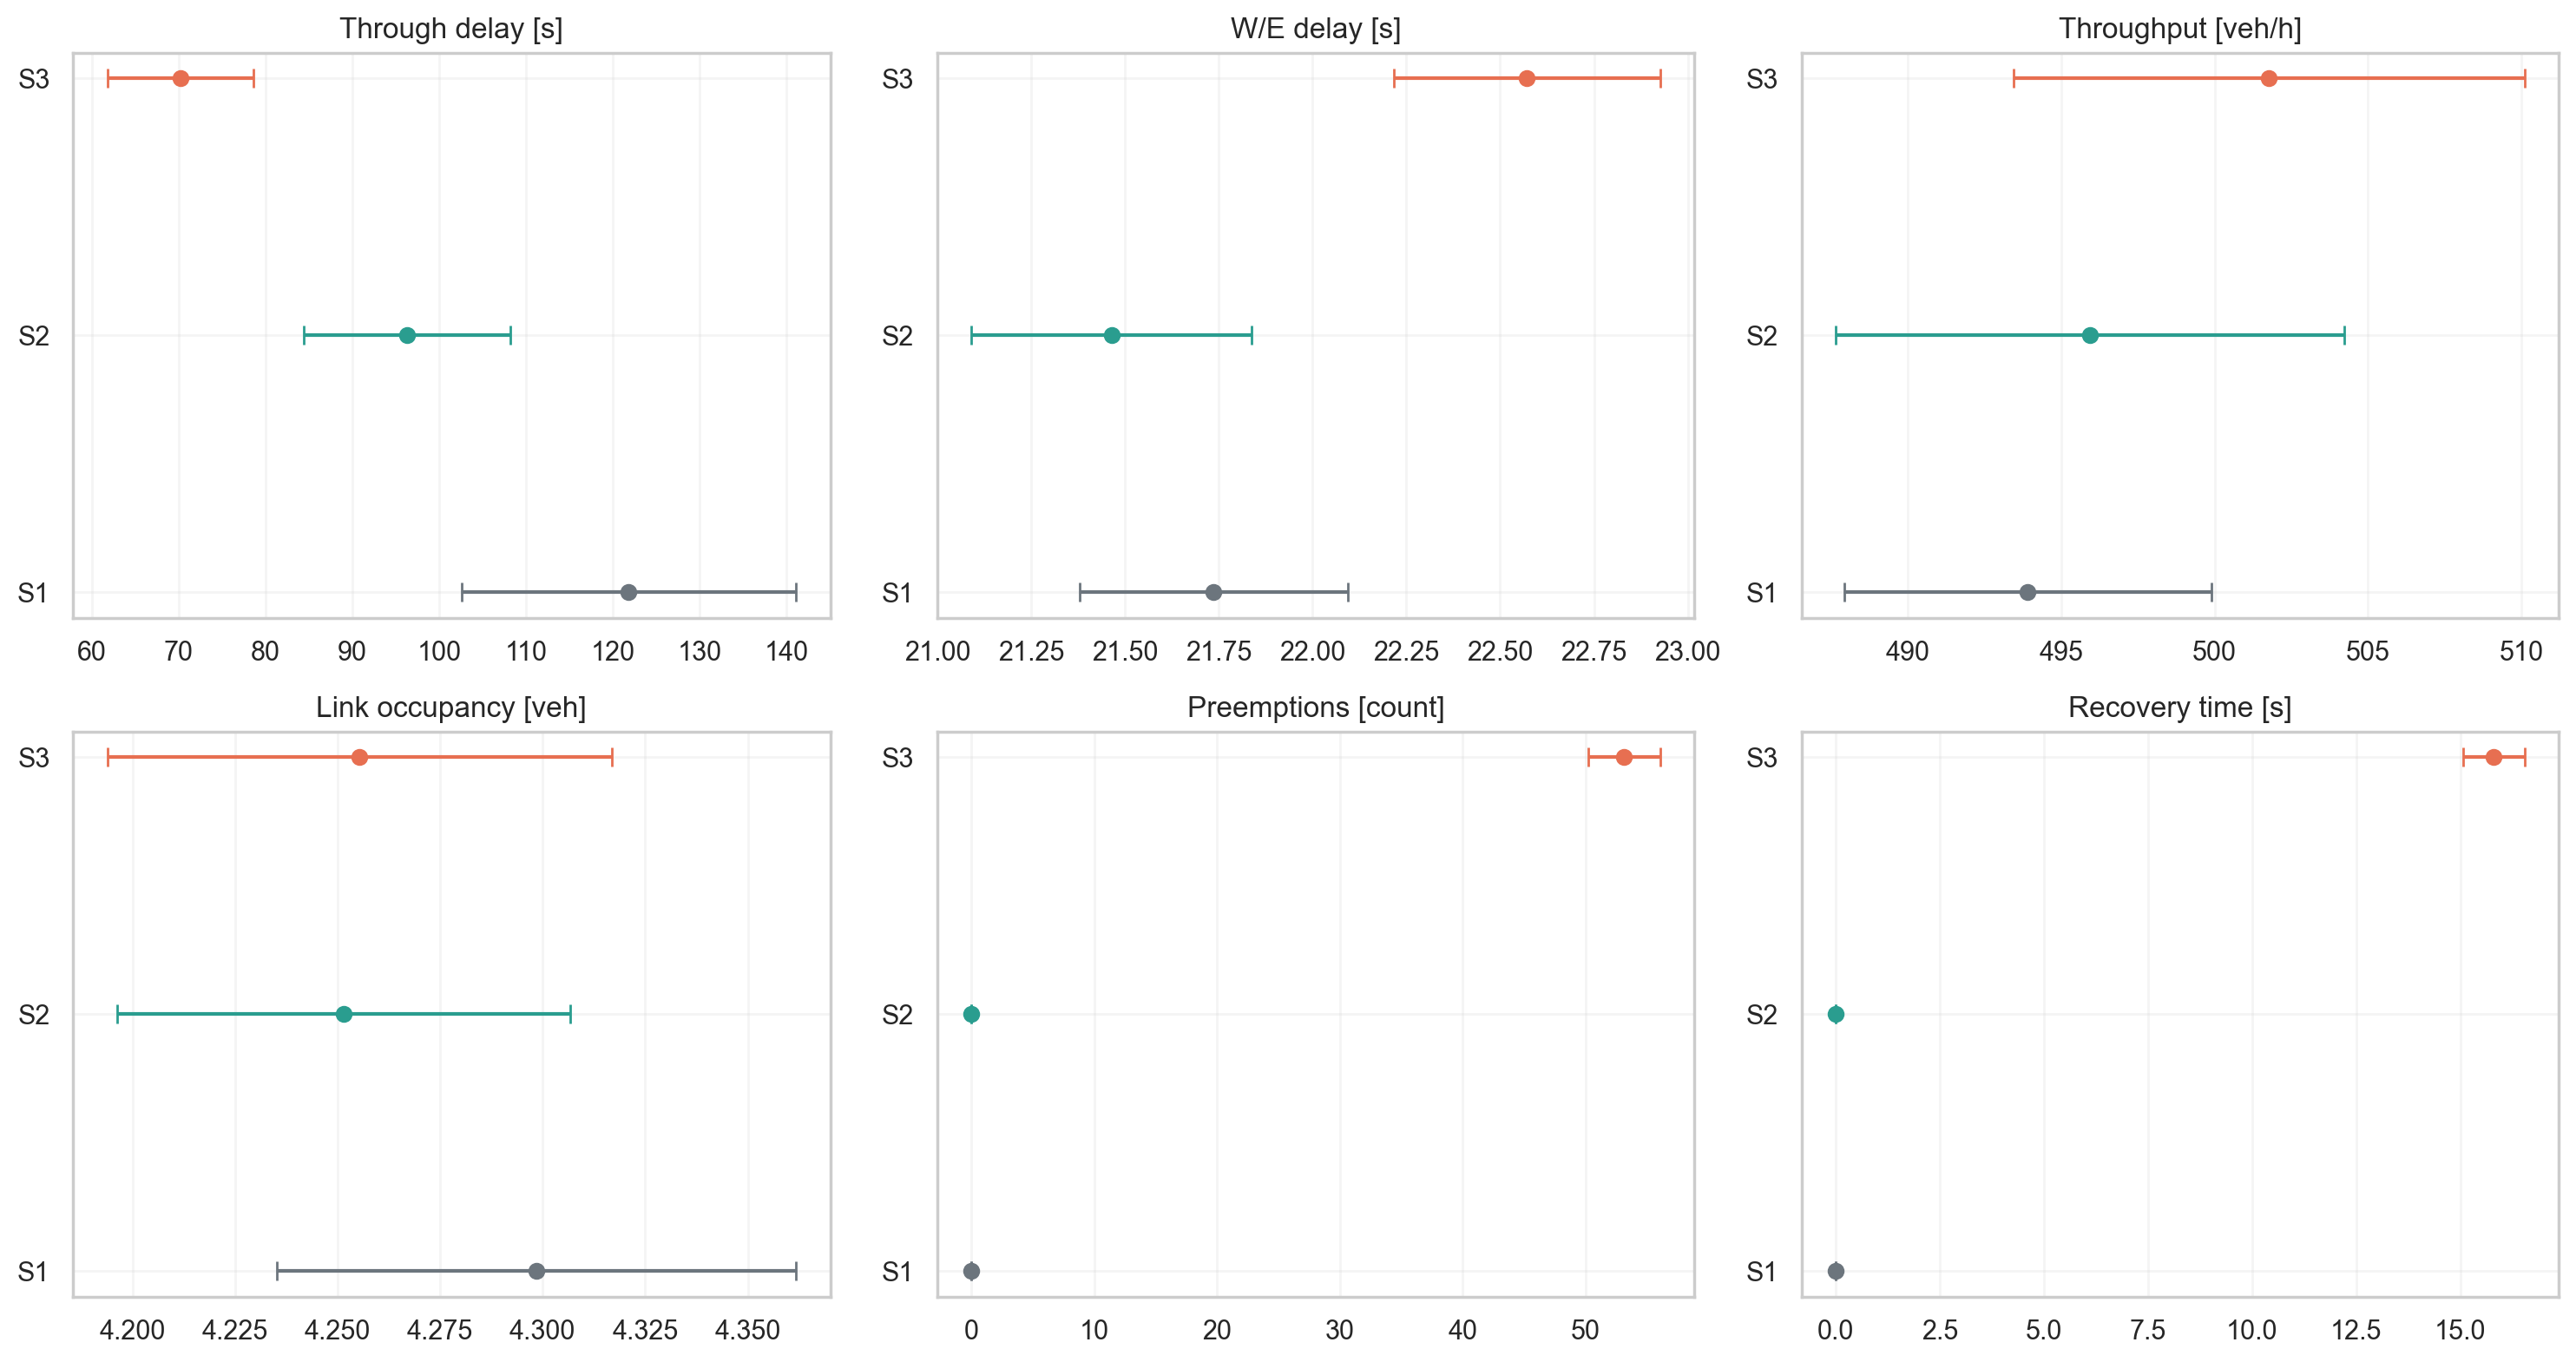
\includegraphics[width=\textwidth]{outputs/fig_ci_comparison.png}
\caption{95\,\% confidence-interval comparison for the main KPIs across the three scenarios. The horizontal bars represent the CI width; dots mark replication means.}
\label{fig:ci}
\end{figure}

\begin{figure}[H]
\centering
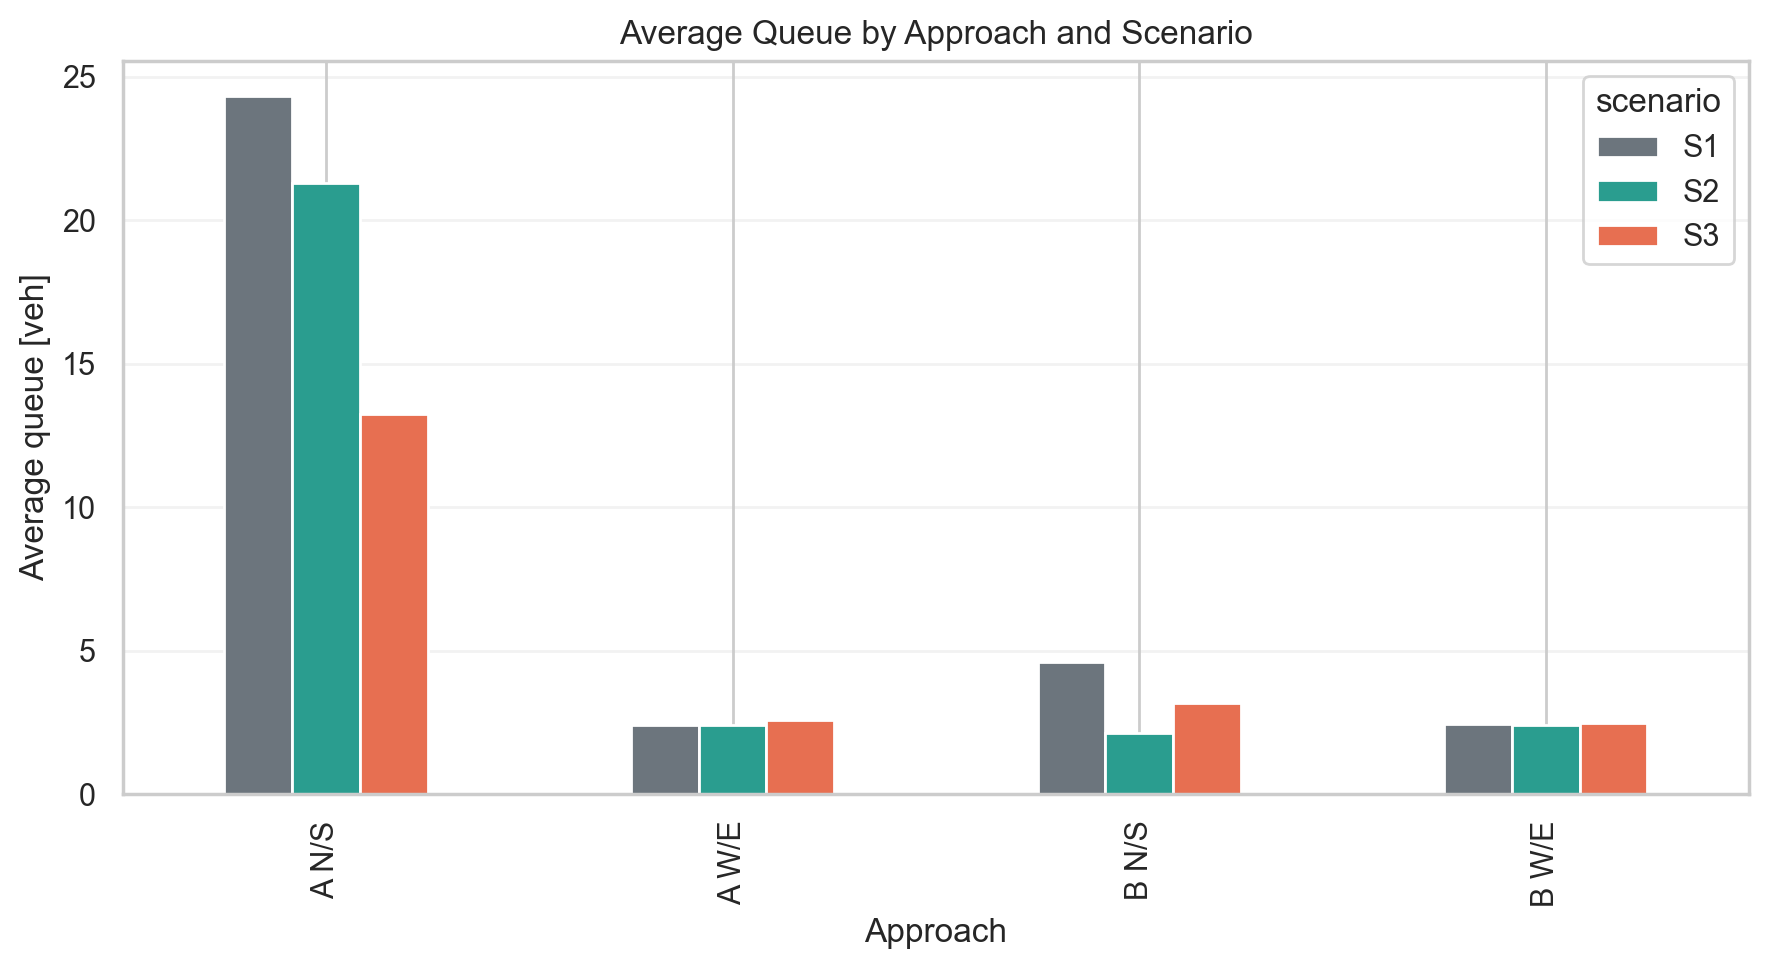
\includegraphics[width=\textwidth]{outputs/fig_queue_profile.png}
\caption{Queue-profile comparison across scenarios, showing both average and maximum queue lengths for every approach.}
\label{fig:queue}
\end{figure}

% ══════════════════════════════════════════════════════════════════
%  4. COMPARATIVE DISCUSSION
% ══════════════════════════════════════════════════════════════════
\section{Comparative Discussion}
\label{sec:discussion}

\subsection{Effect of Coordination (S1 vs.\ S2)}

\begin{findingbox}[Key Finding]
Coordination reduces southbound through-delay by \textbf{21.4\,\%} and cuts the average B\,N/S queue by \textbf{55.9\,\%}.
\end{findingbox}

This is the main benefit expected from a 20\,s offset: vehicles released from~A arrive at~B closer to the start of B's N/S green, thereby encountering shorter queues and less red-time waiting. The throughput effect is negligible ($-0.24\,\%$), which suggests that~A remains the practical bottleneck and coordination mainly \emph{reduces waiting} rather than increasing discharge capacity.

\subsection{Effect of Emergency Preemption (S2 vs.\ S3)}

Relative to S2, S3 changes the performance mix rather than hurting every KPI uniformly:

\begin{itemize}[leftmargin=1.2em,itemsep=3pt]
  \item \textbf{Through-delay drops by another 26.3\,\%} because preemptions create bonus N/S green time that also serves non-emergency corridor vehicles waiting behind the emergency unit.
  \item \textbf{W/E delay rises by 6.1\,\%} and A\,W/E average queue rises by 7.7\,\% due to interrupted W/E phases.
  \item \textbf{B\,N/S average queue rises by 59.5\,\%}: preemptions release extra~A platoons that reach~B in bursts and bunch the downstream queue even while corridor delay improves on average.
\end{itemize}

\begin{cautionbox}[Performance Trade-Off]
Emergency preemption improves the priority corridor but does so by \emph{redistributing} delay away from the emergency path and toward interrupted side-street traffic and downstream platoon build-up.
\end{cautionbox}

\subsection{Most Affected KPI}

Among the headline KPIs in Table~\ref{tab:main-kpis}, \textbf{through-delay} shows the largest percentage change between S2 and S3. Among the adverse effects specifically, the most visible degradation is the increase in cross-street delay and the sharp growth of the B\,N/S queue. In other words, preemption improves the priority corridor strictly at the expense of non-priority movements.

% ══════════════════════════════════════════════════════════════════
%  5. VERIFICATION AND VALIDATION
% ══════════════════════════════════════════════════════════════════
\section{Verification and Validation}
\label{sec:vv}

\subsection{Internal Consistency Checks}

We used several sanity checks in the notebook:
\begin{itemize}[leftmargin=1.2em,itemsep=3pt]
  \item Queue lengths and link occupancy remain \emph{non-negative} at all times.
  \item Blocking frequency always lies in $[0,1]$.
  \item Preemption counts are exactly zero in S1 and~S2 while remaining positive in S3.
\end{itemize}
These checks verify that the core bookkeeping and scenario toggles behave as expected.

\subsection{Downstream Blocking Validation}

\begin{infobox}[Blocking Frequency = 0]
In the required scenarios the observed blocking frequency is zero for all 20 replications. This is \textbf{not a coding bug}. With the assignment parameters, A and B have symmetric N/S green times and identical single-server mean service times, so the maximum A$\rightarrow$link discharge rate is effectively the same as the maximum B drain rate. Under that symmetry the link does not fill before A itself becomes the active bottleneck.
\end{infobox}

To validate that spillback logic exists and is correctly coded, we ran a controlled \textbf{stress test} in the notebook with B's N/S green shortened to 10\,s and the link capacity reduced to 20~vehicles. Under that forced-bottleneck case the model produces positive blocking frequency and elevated link occupancy, confirming that the blocking rule is active even though KPI\,5 remains zero in the official scenarios.

\subsection{Experimental-Design Verification}

We verified the experimental design itself:
\begin{itemize}[leftmargin=1.2em,itemsep=3pt]
  \item Replication-level 95\,\% confidence intervals are produced for every KPI.
  \item RNG streams are separated by source (Table~\ref{tab:rng}).
  \item Warm-up treatment is applied consistently to both time-persistent and entity-based metrics.
\end{itemize}
These checks give us confidence that the reported scenario differences are due to model logic rather than bookkeeping artefacts.

% ══════════════════════════════════════════════════════════════════
%  6. CONCLUSION
% ══════════════════════════════════════════════════════════════════
\section{Conclusion}
\label{sec:conclusion}

This study demonstrates that a relatively simple coordination mechanism -- a 20\,s green-wave offset -- materially improves corridor performance by reducing southbound through-delay by over 20\,\% and halving the downstream B\,N/S queue. Emergency preemption further boosts corridor delay performance, but at the cost of increased cross-street delays and downstream queue volatility. The simulation model was verified through internal consistency checks, a dedicated blocking stress test, and proper experimental-design safeguards including independent RNG streams and a rigorous warm-up protocol. Together, these results highlight that signal coordination is an effective but inherently trade-off-laden strategy: corridor efficiency gains come at the expense of non-priority movements, and emergency preemption amplifies this redistribution effect.

\end{document}
